También se le conoce como linea de equilibrio o punto de equilibrio.

Es la posición en la que las partículas de un medio se encontrarían si no hubiera perturbación, es decir, cuando no hay onda.

Es el punto central en torno al cual vibran las parículas de un medio. También se considera la posición antes y después de producirse la vibración.

Se identifica con el eje de las abscisas $x$ en un plano cartesiano.

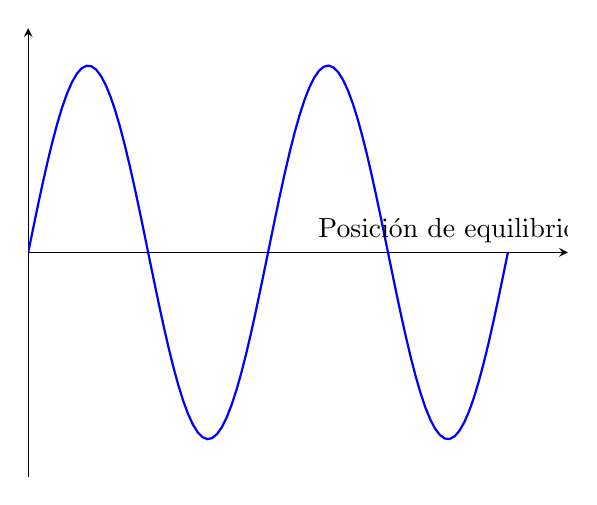
\begin{tikzpicture}
  \begin{axis}[
    xmin=0,xmax=4.5*pi,
    ymin=-1.2,ymax=1.2,
    axis lines=middle,
    xtick={0},
    ytick={0}
    ]

    % Funcion senoidal
    \addplot[color=blue,samples=100,domain=0:4*pi,thick]{sin(deg(x))};

    % Posicion de equilibrio
    \node[above] at (axis cs:7*pi/2,0) {Posición de equilibrio};
  \end{axis}
\end{tikzpicture}
